% this file is called up by thesis.tex
% content in this file will be fed into the main document

%: ----------------------- name of chapter  -------------------------
\chapter{Weryfikacja rozwiązania} % top level followed by section, subsection


%: ----------------------- paths to graphics ------------------------

% change according to folder and file names
\ifpdf
    \graphicspath{{4/figures/PNG/}{4/figures/PDF/}{4/figures/}}
\else
    \graphicspath{{4/figures/EPS/}{4/figures/}}
\fi

%: ----------------------- contents from here ------------------------

Rozdział ten opisuje jak wybrany sposób integracji oraz powstały w ten sposób prototypowy system wpływa na łatwość tworzenia i efektywność aplikacji przetwarzających mowę. Proponowane przykładowe aplikacje to:
\begin{itemize}
	\item Automatyczne dyktando
	\item Lektor RSS
	\item Lektor SMS
	\item Konwerter plików graficznych do tekstowych
\end{itemize}
Każdej z proponowanych aplikacji poświęcono osobny podrozdział, w którym jest zdefiniowany przypadek użycia, przedstawione są wymagania funkcjonalne i niefunkcjonalne oraz przedstawiona jest weryfikacja podejścia.


\section{Automatyczne dyktando}
Jest to aplikacja webowa umożliwiająca użytkownikowi ćwiczenie pisowni w różnych językach. Zasada działania jest bardzo prosta, użytkownik ładuje plik tekstowy lub graficzny na serwer oraz wybiera język docelowy, następnie zostaje przekierowany na stronę zawierającą formularz do pisania tekstu oraz odtwarzacz. Użytkownik słucha tekstu i zapisuje w polu tekstowym transkrypcję. W momencie w którym zatwierdzi formularz zostaje on przesłany na serwer i porównany z oryginalnym plikiem wejściowym, w efekcie użytkownik otrzymuje informację o ilości popełnionych błędów oraz o wyrazach które źle zapisał. 
\newpage
\subsection{Przypadek użycia}
\begin{figure}[!h]
	\centering
	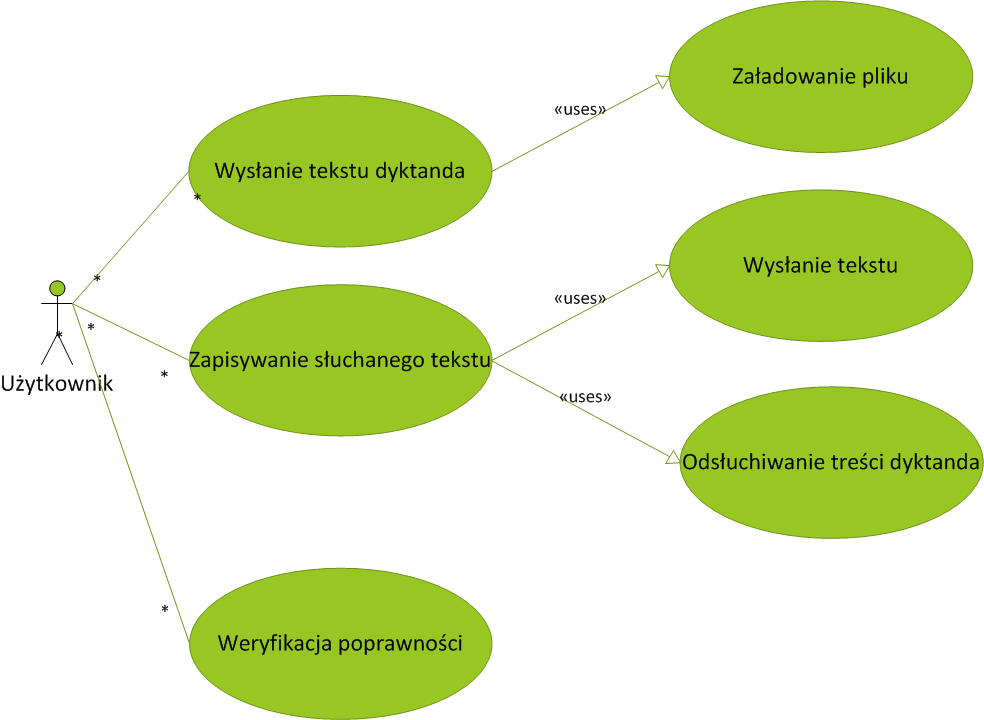
\includegraphics[scale=0.45]{useCaseDictando.png} 
	\caption{Przypadek użycia - Automatyczne dyktando }
\end{figure}

\subsection{Wymagania}
\subsubsection{Wymagania funkcjonalne}
\begin{enumerate}
	\item Obsługiwanie wielu języków
	\item Możliwość podania tekstu źródłowego
		\begin{enumerate}
			\item jako plik graficzny
			\item jako plik tekstowy, wysyłany na serwer
		\end{enumerate}
	\item Umożliwienie użytkownikowi odsłuchania wysłanego tekstu w wybranym przez niego języku
	\item Umożliwienie użytkownikowi wprowadzania tekstu jednocześnie z odsłuchiwaniem
	\item Wygenerowanie i wyświetlenie raportu o ilości błędów popełnionych przez użytkownika
\end{enumerate}

\subsubsection{Wymagania niefunkcjonalne}
\begin{enumerate}
	\item Bezpieczeństwo - użytkownik i tylko on powinien móc widzieć swoje wyniki
	\item Wydajność - dyktowanie tekstu powinno przebiegać płynnie, opóźnienie może występować tylko przed rozpoczęciem, od 0 do 60 sekund, przerwy w czasie dyktowania tekstu są niedopuszczalne
	\item Niezawodność - użytkownik powinien zawsze otrzymać wynik który jest poprawny, tzn. pokazuje dokładną ilość błędów popełnionych przez użytkownika
\end{enumerate}

\subsection{Weryfikacja podejścia}
Jak widać w powyższym podrozdziale wymagania stawiane przed aplikacją są precyzyjne i klarowne. Zastosowane podejście integracyjne sprawia, że stworzenie aplikacji spełniającej wymagania staje się proste. Zapewnienie obsługi wielu języków nie wymaga praktycznie żadnego nakładu pracy ze strony programisty aplikacji klienckiej. Jak zostało to opisane w rozdziale drugim, przy zastosowanym podejściu wystarczy wygenerować i przesłać plik xml z informacją dotyczącą języka docelowego, działa to niezależnie od języka w którym jest tekst wejściowy (pod warunkiem, że w pliku konfiguracyjnym ustawi się tag odpowiedzialny za serwis rozpoznający język). Podobnie przesłanie pliku graficznego, również wymaga tylko umieszczenia odpowiedniego tagu w pliku xml celem wywolania serwisu OCR. Jak łatwo zauważyć wygenerowanie i przesłanie pliku xml nie jest dużym wyzwaniem programistycznym.Widać to szczególnie gdyby porównać to z implementacją bez wykorzystania systemu opartego o rozwiązanie opisane w tej pracy. Musiałaby ona łączyć się z kilkoma zewnętrznymi serwisami, z których każdy prawdopodobnie miałby inny interfejs, konwertować różne formaty plików, obsługiwać błędy itd. Jedyną przewagą osobnej implementacji mogłabybyć szybkość działania, ale i tak różnica nie byłaby duża i sprowadzałaby się głównie do czasu potrzebnego na przesyłanie danych do i z systemu (oczywiście zakładając, że zarówno implementacja platformy jak i aplikacji korzystałaby z tych samych zewnętrznych serwisów). 
Jak widać, w tym przypadku, zastosowane podejście w sposób znaczący pozytywnie wpływa na łatwość i szybkość implementacji aplikacji klienckiej. \\

\section{Lektor SMS}
Jest to aplikacja przeznaczona dla systemu operacyjnego Android. Jak nazwa wskazuje jej funkcjonalność pozwala odczytywać na głos wiadomości tekstowe. Może okazać się bardzo przydatna w czasie jazdy samochodem, wiadomo, że używanie telefonu komórkowego jest zabronione z powodu bezpieczeństwa, tym bardziej, używanie rąk i skupianie wzroku na odczytywanej wiadomości tekstowej jeszcze w większym stopniu niż rozmowa przez telefon prowadzi do odwrócenia uwagi kierowcy od sytuacji na drodze.
Zasada działania tej aplikacji jest bardzo prosta, mianowicie po włączenie przechwytuje ona każde zdarzenie oznaczające otrzymanie wiadomości tekstowej, pobiera jej treść i zamienia ją na dzwięk w dowolnym, wybranym przez użytkownika języku. Co warte zauważenia aplikacja ta ma dwa różne sposoby generowania mowy:
\begin{itemize}
	\item korzystając z usług udostępnianych przez przykładową implementację systemu integrującego usługi przetwarzania mowy
	\item korzystając z wbudowengo w system Android TTS'a
\end{itemize} 
Dzięki wykorzystaniu obu rozwiązań mamy możliwość bezpośredniego porównania. Wybór sposobu generowania dzwięku zależy od dostępności połączenia z internetem, jeżeli takie istnieje to aplikacja korzysta z zewnętrznego systemu, w przeciwnym razie wykorzystuje wbudowany TTS. Oczywiście użytkownik ma możliwość ustawienia dla których numerów aplikacja będzie działać.
\newpage
\subsection{Przypadek użycia}
\begin{figure}[!h]
	\centering
	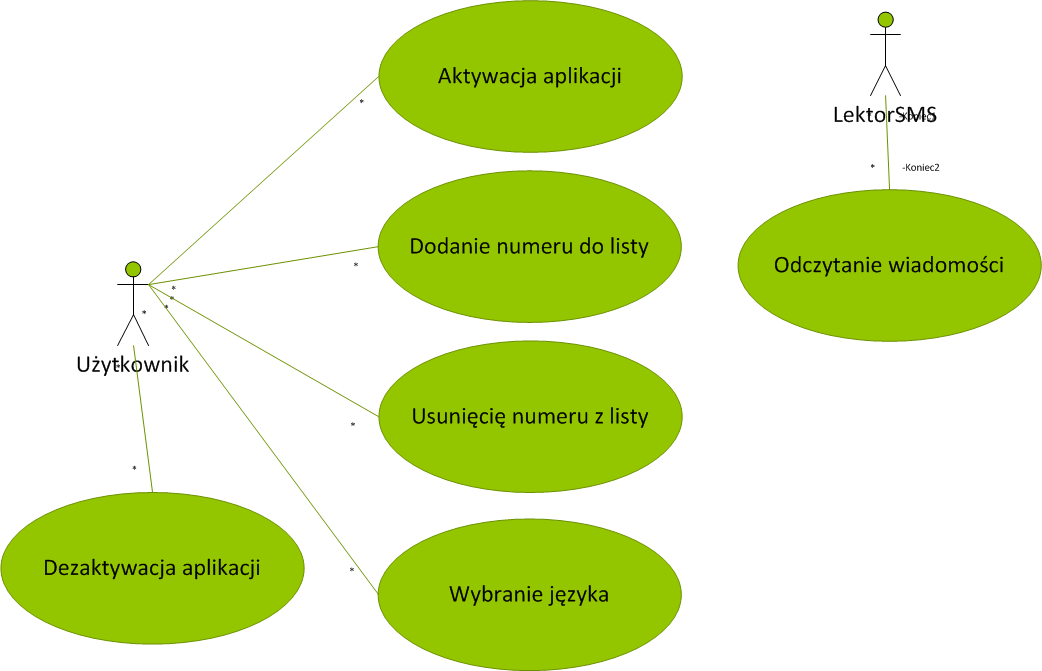
\includegraphics[scale=0.45]{useCaseLektorSMS.png} 
	\caption{Przypadek użycia - LektorRSS}
\end{figure}

\subsection{Wymagania}
\subsubsection{Wymagania funkcjonalne}
\begin{enumerate}
	\item Możliwość aktywacji i dezaktywacji aplikacji
	\item Możliwość ustawienia języka w którym będzie odczytywana treść wiadomości
	\item Możliwość filtrowania obsługiwanych wiadomości SMS po numerach nadawców 
	\item Obsługiwanie więcej niż jednego języka wiadomości
	\item Automatyczne odczytywanie otrzymanych wiadomości
\end{enumerate}
\subsubsection{Wymagania niefunkcjonalne}
\begin{enumerate}
	\item Dostęp do apikacji musi być chroniony hasłem
	\item Użyteczność - poprawne działanie na dowolnym urządzeniu z systemem Android z dostępem do siecii lub z systemem w wersji co najmniej 1.6
\end{enumerate}

\subsection{Weryfikacja podejścia}
Wykorzystanie sposobu integracji systemów przetwarzania mowy rozważanego w tej pracy pozwala na bardzo łatwą implementację aplikacji spełniającej wszystkie stawiane przed nią wymagania. Co więcej pozwala ona na łatwą rozbudowę. Można na przykład dodać funkcjonalność polegającą na tłumaczenie wiadomości na konkretny język docelowy, co w implementacji bez wykorzystania systemu byłoby dużo trudniejsze i wymagało przesłania większej ilości danych co ponosi za sobą koszty(szczególnie jeżeli telefon działa w roamingu). Z drugiej strony system Android daje dostęp do wbudowanej usługi TTS. Jest ona dość dobrej jakości, również obsługuje kilka języków, co więcej nie wymaga dostępu do internetu co jest jej dużym plusem. Ci więcej implemetancja aplikacji z jej wykorzystaniej również jest prostym zadaniem. Co więcej aplikacja, korzystająca z natywnego TTS'a będzie napewno szybsza. Na podstawie wszystkich argumentów można dojść do wniosku, że w tym przypadku nie ma potrzeby korzystania z koncepcyjnego systemu. Dlatego też, w tym konkretnym przypadku, ciężko ocenić które rozwiązanie jest lepsze. Wszystko zależy od tego czy ważniejsza jest jakość wygenerowanego dźwięku, możliwość dodania dodatkowych funkcji czy szybkość działania i nie obciążanie połączenia internetowego.

\section{Lektor RSS}
Jest to aplikacje webowa której zadaniem jest odczytywanie wiadomości RSS ze źródeł podanych przez użytkownika, może on podać źródło przez specjalny formularz, załadować plik tekstowy zawierający adresy źródeł. Niezależnie od użytej metody można podać język wiadomości lub też użyć serwisu rozpoznającego. Możliwe jest również przetłumaczenie wiadomości na język podany przez użytkownika i dopiero wtedy przeczytanie jej przez odpowiedniego lektora. Użytkownik ma również możliwość ustawienia co jaki czas ma następować sprawdzanie źródła celem znalezienia nowych wiadomości.	 
\newpage
\subsection{Przypadek użycia}
\begin{figure}[!h]
	\centering
	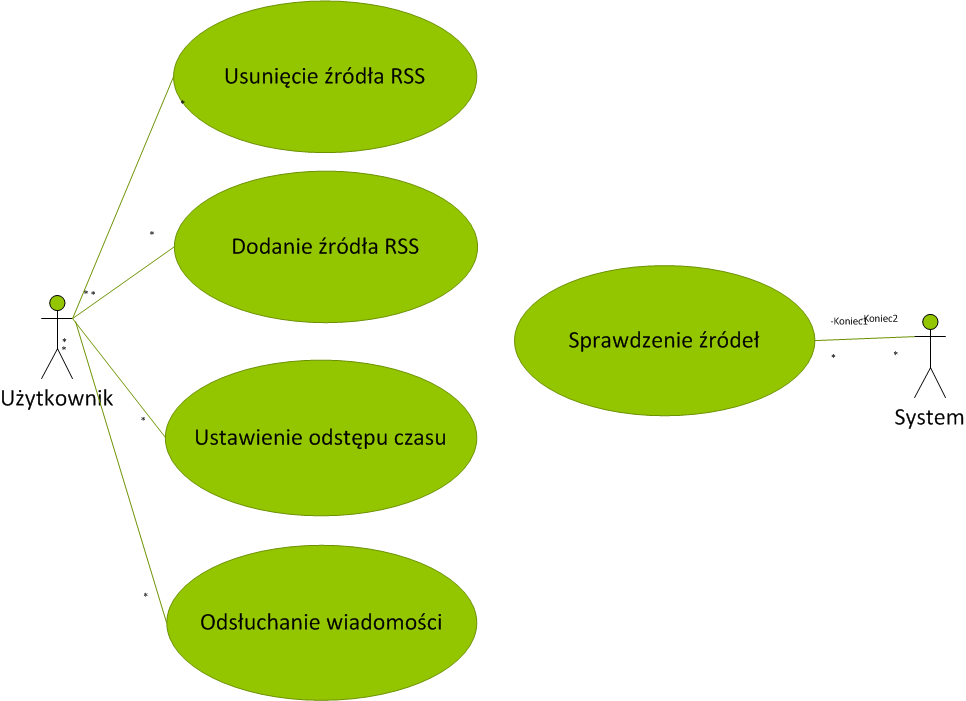
\includegraphics[scale=0.45]{useCaseRSS.png} 
	\caption{Przypadek użycia - LektorRSS}
\end{figure}

\subsection{Wymagania}
\subsubsection{Wymagania funkcjonalne}
\begin{enumerate}
	\item Możliwość dodania źródła RSS
	\item Możliwość usunięcia źródła RSS
	\item Obsługiwanie więcej niż jednego języka wiadomości
	\item Automatyczne sprawdzanie czy któreś ze źródeł nie zawiera nowej wiadomości
	\item Możliwość ustawienia odstępów czasowych pomiędzy sprawdzaniem przez system źródeł
	\item Automatyczne Odczytanie użytkownikowi nowych wiadomości (w przypadku istnienia) 
\end{enumerate}  
\subsubsection{Wymagania niefunkcjonalne}
\begin{enumerate}
	\item Niezawodność - system nie może pominąć żadnej wiadomości z listy źródeł zdefiniowanej przez użytkownika
	\item Szybkość - różnica czasu pomiędzy udostępnieniem nowej wiadomości w którymś ze źródeł a otrzymaniem jej przez użytkownika nie może przekraczać czasu pomiędzy sprawdzeniami w poszukiwaniu uaktualnień (czas ten ustawia użytkownik)
	\item Możliwość personalizacji - użytkownik powinien móc dodać dowolną ilość różnych źródeł, system powinien zapewnić ich niepowtarzalność(usuwać duplikaty)
\end{enumerate}

\subsection{Weryfikacja podejścia}
Tak jak w sekcji opisującej aplikację Automatyczne Dyktando wymagania przedstawione powyżej są jasne i klarowne. Po raz kolejny zastosowane podejście integracyjne sprawia, że napisanie aplikacji klienckiej, spełniającej wymagania przed nią stawiane jest proste. Dzięki użyciu ESB i oferowanych przez niego endpointów jest możliwe przerzucenie konieczności pobierania wiadomości ze źródeł RSS na stronę systemu. Podobnie jak w przypadku aplikacji opisanej wyżej zarówno rozpoznawanie języka, tłumaczenie czy generowanie mowy w odpowiednim języku nie stanowi dla programisty, autora aplikacji klienckiej żadnego problemu, wystarczającym jest wygenerowanie pliku xml zawierającego odpowiednie instrukcje. Implementacja podobnej, równie rozbudowanej aplikacji, bez wykorzystania systemu integrującego serwisy odpowiadające za przetwarzanie mowy byłaby trudniejsza oraz wymagałaby poświęcenia większej ilości czasu. Poza problemami podobnymi do tych jakie były opisane w przypadku Aumatycznego Dyktanda dochodzi jeszcze sprawa pobierania RSS'ów, ich parsowania itd. Pozostałe wymagania, takie jak bezpieczeństwo czy też konieczność przechowywania danych w bazie danych muszą być zaspokojone w ten sam sposób niezależnie od wykorzystania systemu. \\
W przypadku tej aplikacji również klarownym jest fakt, że zastosowane podejście bardzo upraszcza implementację.


% ---------------------------------------------------------------------------
%: ----------------------- end of thesis sub-document ------------------------
% ---------------------------------------------------------------------------

